
%(BEGIN_QUESTION)
% Copyright 2010, Tony R. Kuphaldt, released under the Creative Commons Attribution License (v 1.0)
% This means you may do almost anything with this work of mine, so long as you give me proper credit

Calculate the appropriate LRV and URV pressures for this hydrostatic level measurement system, assuming the process liquid has a weight density of 43 pounds per cubic foot at the typical operating temperature of 120 degrees Fahrenheit:

$$\includegraphics[width=15.5cm]{i04514x01.eps}$$

\vskip 20pt \vbox{\hrule \hbox{\strut \vrule{} {\bf Suggestions for Socratic discussion} \vrule} \hrule}

\begin{itemize}
\item{} Suppose an instrument technician relocates the DP transmitter to a location that is {\it lower} than it is right now, from 10 feet below the LRV to 15 feet below the LRV.  Will the transmitter still accurately register liquid level in the vessel?  If not, determine whether the error will be {\it high} (indicating more liquid than there actually is) or {\it low} (indicating less liquid than there actually is).
\item{} Suppose an instrument technician relocates the DP transmitter to a location that is {\it higher} than it is right now, from 10 feet below the LRV to 2 feet above the LRV.  Will the transmitter still accurately register liquid level in the vessel?  If not, determine whether the error will be {\it high} (indicating more liquid than there actually is) or {\it low} (indicating less liquid than there actually is).
\item{} Suppose the DP transmitter is replaced with another having a denser fill fluid (1.85 instead of 1.07).  Will the transmitter still accurately register liquid level in the vessel?  If not, determine whether the error will be {\it high} (indicating more liquid than there actually is) or {\it low} (indicating less liquid than there actually is).
\item{} Suppose some of the fill fluid leaks out of the ``low'' side capillary tube.  Will the transmitter still accurately register liquid level in the vessel?  If not, determine whether the error will be {\it high} (indicating more liquid than there actually is) or {\it low} (indicating less liquid than there actually is).
\item{} Suppose the ambient temperature dramatically increases, causing the fill fluid to expand inside both capillary tubes.  Will the transmitter still accurately register liquid level in the vessel?  If not, determine whether the error will be {\it high} (indicating more liquid than there actually is) or {\it low} (indicating less liquid than there actually is).
\end{itemize}

\underbar{file i04514}
%(END_QUESTION)





%(BEGIN_ANSWER)

LRV = $-198.1$ inches H$_{2}$O \hskip 50pt URV = $-107.1$ inches H$_{2}$O

%(END_ANSWER)





%(BEGIN_NOTES)

Since both capillary tubes are filled with the same fill fluid (SG = 1.07), we can safely ignore any suppression common to both -- i.e. the bottom 10 feet cancel out.  In other words, we can proceed with this problem as if the transmitter were located at the same height as the bottom remote seal, with a wet compensating leg 18 feet tall (216 inches).

\vskip 10pt

LRV = 4 ft of process fluid $-$ 18 ft of fill fluid = (48 in)(43/62.428) $-$ (216 in)(1.07) = $-198.1$ inches H$_{2}$O

URV = 15 ft of process fluid $-$ 18 ft of fill fluid = (180 in)(43/62.428) $-$ (216 in)(1.07) = $-107.1$ inches H$_{2}$O 

\vskip 10pt

The static pressure of 83 PSI is completely irrelevant to the LRV/URV calculations.  The 120 $^{o}$F temperature value could be relevant, but only if it changes enough to cause the fluid densities to substantially change.

The 10 foot suppression is also irrelevant to the calculations, because those 10 feet of capillary tube on each side of the transmitter contain the same type of fill fluid, and therefore their respective hydrostatic pressures cancel at the DP transmitter.

%INDEX% Measurement, level: hydrostatic pressure

%(END_NOTES)

